%=== NOTE: Use \chapter to introduce each new appendix.

% TODO: MAYBE DON'T INCLUDE ANY \section or \subsection content!
% TODO: Clean all this up!

\chapter{Ad hoc impact parameter studies}
\label{app:adhoc_studies}

% \chapter{The sign of impact parameter}
% \label{app:qd0_derivation}

Consider a reconstructed muon track projected onto the $x$-$y$ plane, transverse to the beam pipe.
If the muon were prompt, then it truly would have originated from the primary vertex (PV).
However, due to inefficiencies in reconstructing the muon track, 
the best-fit track may not intersect the PV. 

Looking at Fig.~\ref{fig:traj} (A), the (very exaggerated) muon track is represented by the black circle.
This track could either be a $\Pmu^+$ (blue arrowheads) travelling around clockwise, since the magnetic field points along the $+z$ direction,
or it could represent the track of a $\Pmu^-$ (orange arrowheads) travelling counterclockwise.
From the figure it can be seen that:
\begin{itemize}
    \item $\vec{s} =$ the vector which begins at the PV (the origin) and ends at the point-of-closest-approach (PCA) along the muon track.
    \item $\phi_s =$ the azimuthal angle of ${\vec{s}}$ as measured from the $x$ axis.
    \item $\phi_{\Pmu^{\pm}} =$ the azimuthal angle of the $\vec{p}_{T,\Pmu^{\pm}}$, tangent to the track at the PCA, measured from the $x$ axis.
\end{itemize}
%%%%%%%%%%%%%%%%%%%%
\begin{multiFigure}
    \centering
    \addFigure{0.49}{figures/adhoc_d0/PV_outside.png}
    \addFigure{0.49}{figures/adhoc_d0/PV_inside.png}
        \captionof{figure}
            [Diagram showing circular trajectory of a muon with respect to the primary vertex]
            {Diagram showing circular trajectory of a muon with respect to the primary vertex.
            \;A) The true primary vertex (PV) is \emph{outside} the circular trajectory of a muon.
            \;B) The PV is \emph{inside} the circular trajectory of a muon.
            } 
        \label{fig:traj}
\end{multiFigure}
%%%%%%%%%%%%%%%%%%%%

From Fig.~\ref{fig:traj} (Left) we see that:
\begin{equation}
    \label{azimuth}
\phi_{\Pmu^{\pm}} = \phi_{s} \pm \pi/2.
\end{equation}
Using one possible definition of $d_{0}$ and Eqn.~\ref{azimuth} shows that 
the $d_0$ for $\Pmu^{\pm}$ which came from a PV outside the circle trajectory is:
\begin{align*}
    d_{0,\Pmu^{\pm}}^{\text{PV,outside}} &= -x \sin{( \phi_{\Pmu^{\pm}} )}  + y \cos{( \phi_{\Pmu^{\pm}} )} \\
    &= - x \sin{( \phi_s \pm \pi/2 )} + y \cos{( \phi_s \pm \pi/2 )}  \\
    &= -x \big[ \sin{(\phi_s)} \cos{(\pi/2)}  \pm \sin{(\pi/2)} \cos{(\phi_s)} \big]  
       + y \big[\cos{(\phi_s)} \cos{(\pi/2)} \mp \sin{(\phi_s)} \sin{(\pi/2)} \big] \\
    &= - x [\pm \cos{(\phi_s)}] + y [\mp \sin{(\phi_s)}] \\
    &= \mp [x \cos{(\phi_s)}  + y \sin{(\phi_s)}] \\
    &= \mp \big[ x \hat{x} + y \hat{y}  \big] \boldsymbol{\cdot} \big[ \cos(\phi_{s}) \hat{x} + \sin(\phi_{s}) \hat{y}  \big] \\
    &= \mp \vec{s} \boldsymbol{\cdot} \hat{s} \\
    &= \mp \lvert \vec{s} \rvert   \lvert \hat{s} \rvert    \cos{(0)}
\end{align*}
\begin{equation}
    \label{eqn:d0_out}
    \implies  d_{0,\Pmu^{\pm}}^{\text{PV,outside}} = \mp \lvert \vec{s} \rvert. 
\end{equation}

The case for the PV being {\it inside} the circle trajectory (Fig.~\ref{fig:traj}, Right) simply leads to a sign change in Eqn.~\ref{azimuth}:
\begin{equation}
    \label{azimuth_flipped}
\phi_{\Pmu^{\pm}} = \phi_{s} \mp \pi/2.
\end{equation}
Starting again from the definition of $d_0$, but this time using Eqn.~\ref{azimuth_flipped}, ultimately gives:
\begin{equation}
    \label{eqn:d0_in}
\implies  d_{0,\Pmu^{\pm}}^{\text{PV,inside}} = \pm \lvert \vec{s} \rvert.
\end{equation}

Indeed we see that the magnitude of $d_0$ {\it is the transverse impact parameter} $(\lvert \vec{s} \rvert)$, as expected!
The sign of $d_0$, however, is not possible to interpret at this point: 
for a $d_0 > 0$ could either mean a $\Pmu^-$ coming from a PV outside the circlular trajectory \emph{or}
could mean a $\Pmu^+$ coming from a PV found inside the circle.

Since the sign of $d_0$ is not useful by itself, consider multiplying $d_0$ by the charge of its corresponding muon. 
We then see that Eqn.~\ref{eqn:d0_out} becomes:
\begin{align*}
    {\rm charge}(\Pmu^{\pm}) \cdot d_{0,\Pmu^{\pm}}^{\text{PV,outside}} &= \pm1 \cdot \mp \lvert \vec{s} \rvert \\
    &= - \lvert \vec{s} \rvert < 0,
\end{align*}
which is always negative. Similarly, Eqn.~\ref{eqn:d0_in} gives the opposite result:
\begin{equation*}
    {\rm charge}(\Pmu^{\pm}) \cdot d_{0,\Pmu^{\pm}}^{\text{PV,inside}} = + \lvert \vec{s} \rvert > 0,
\end{equation*}
which of course is always positive. 

Therefore, if we know the sign of the muon (say, negative) 
and the sign of its $d_0$ (say, positive), 
then we can simply take the product (negative in this case) 
and infer that the PV must have been \emph{outside} the muon trajectory!

To summarize: it is the \emph{product} of the charge and $d_0$ that contains useful information about the muon track. 
\[
    {\rm PV} = 
\begin{cases}
    \text{inside of circle},& \text{if charge}(\Pmu^{\pm}) \cdot d_{0,\Pmu^{\pm}} > 0 \\
    \text{outside of circle},& \text{if charge}(\Pmu^{\pm}) \cdot d_{0,\Pmu^{\pm}} < 0.
\end{cases}
\]




%---------------%
% \newpage
\chapter{Correlation between transverse momentum bias and impact parameter}
% \label{app:dpT_graphs}

% TODO: Make multiFigure
\begin{multiFigure}
    \centering
    \addFigure{0.45}{figures/adhoc_d0/dpToverpTvsqd0_final_plots_2017/graph_dpTvsqd0_0p0eta0p2.pdf}
    \addFigure{0.45}{figures/adhoc_d0/dpToverpTvsqd0_final_plots_2017/graph_dpTvsqd0_0p2eta0p4.pdf}
    \addFigure{0.45}{figures/adhoc_d0/dpToverpTvsqd0_final_plots_2017/graph_dpTvsqd0_0p4eta0p6.pdf}
    \addFigure{0.45}{figures/adhoc_d0/dpToverpTvsqd0_final_plots_2017/graph_dpTvsqd0_0p6eta0p8.pdf}
    \addFigure{0.45}{figures/adhoc_d0/dpToverpTvsqd0_final_plots_2017/graph_dpTvsqd0_0p8eta1p0.pdf}
    \addFigure{0.45}{figures/adhoc_d0/dpToverpTvsqd0_final_plots_2017/graph_dpTvsqd0_1p0eta1p2.pdf}
    \addFigure{0.45}{figures/adhoc_d0/dpToverpTvsqd0_final_plots_2017/graph_dpTvsqd0_1p2eta1p5.pdf}
    \captionof{figure}
        [\pTmismeas vs. avg$(\qdzero)$ for 2017 MC in bins of \abseta: 0.0--0.2--0.4--0.6--0.8--1.0--1.25--1.5]
        {Plots of \pTmismeas vs. avg$(\qdzero)$ for 2017 MC.
        The \abseta bin edges used are: [0.0--0.2--0.4--0.6--0.8--1.0--1.25--1.5].
        Each line uses data from a single \pT bin. 
        The \pT correction parameters for each (\abseta, \pT) bin are found in the legend.
    }
\end{multiFigure}
\newpage
% % TODO: Make multiFigure
% \begin{figure}[!htbp]
%     % \vspace*{0.3cm}
%     \centering
%     { \includegraphics[height=4cm]{../../higgsmassmeasurement/AN-19-248/Figures/adhoc_d0/dpToverpTvsqd0_graphs_2017/graph_dpTvsqd0_1p5eta1p8.png}}
%     { \includegraphics[height=4cm]{../../higgsmassmeasurement/AN-19-248/Figures/adhoc_d0/dpToverpTvsqd0_graphs_2017/graph_dpTvsqd0_1p8eta2p0.png}}
%     { \includegraphics[height=4cm]{../../higgsmassmeasurement/AN-19-248/Figures/adhoc_d0/dpToverpTvsqd0_graphs_2017/graph_dpTvsqd0_2p0eta2p1.png}}
%     { \includegraphics[height=4cm]{../../higgsmassmeasurement/AN-19-248/Figures/adhoc_d0/dpToverpTvsqd0_graphs_2017/graph_dpTvsqd0_2p1eta2p2.png}}
%     { \includegraphics[height=4cm]{../../higgsmassmeasurement/AN-19-248/Figures/adhoc_d0/dpToverpTvsqd0_graphs_2017/graph_dpTvsqd0_2p2eta2p3.png}}
%     { \includegraphics[height=4cm]{../../higgsmassmeasurement/AN-19-248/Figures/adhoc_d0/dpToverpTvsqd0_graphs_2017/graph_dpTvsqd0_2p3eta2p4.png}}
%     \caption
%         [Graphs of \pTmismeas vs. avg$(\qdzero)$ for 2017 MC: bins = [1.5, 1.75, 2.0, 2.1, 2.2, 2.3, 2.4].]
%         { Graphs of \pTmismeas vs. avg$(\qdzero)$ for each \abseta bin using 2017 MC.
%         The \abseta bin edges shown above are: $[1.5, 1.75, 2.0, 2.1, 2.2, 2.3, 2.4]$.
%         Each line uses data from a single \pT bin. 
%         The \pT correction parameters for each (\abseta, \pT) bin are found in the legend.
%     }
% \end{figure}

% \newpage
% % TODO: Make multiFigure
% \begin{figure}[!htbp]
%     % \vspace*{0.3cm}
%     \centering
%     { 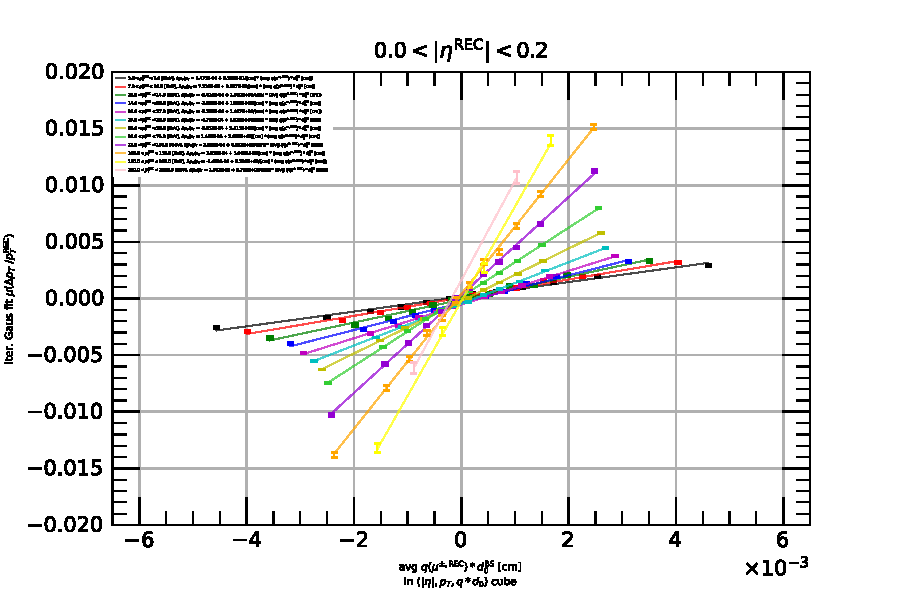
\includegraphics[height=4cm]{../../higgsmassmeasurement/AN-19-248/Figures/adhoc_d0/dpToverpTvsqd0_graphs_2018/graph_dpTvsqd0_0p0eta0p2.png}}
%     { 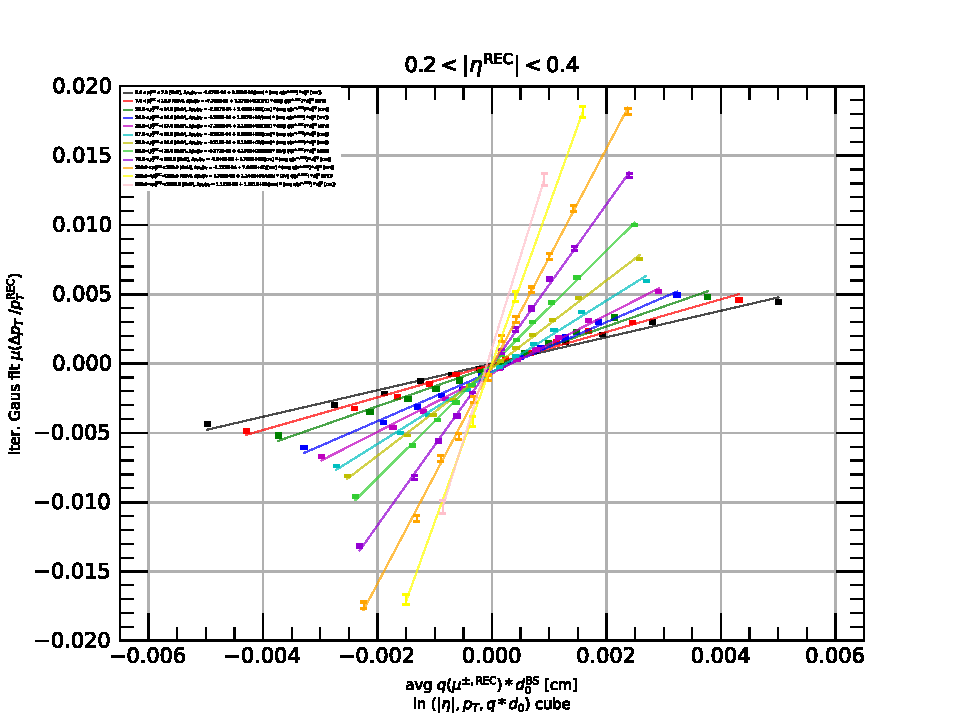
\includegraphics[height=4cm]{../../higgsmassmeasurement/AN-19-248/Figures/adhoc_d0/dpToverpTvsqd0_graphs_2018/graph_dpTvsqd0_0p2eta0p4.png}}
%     { 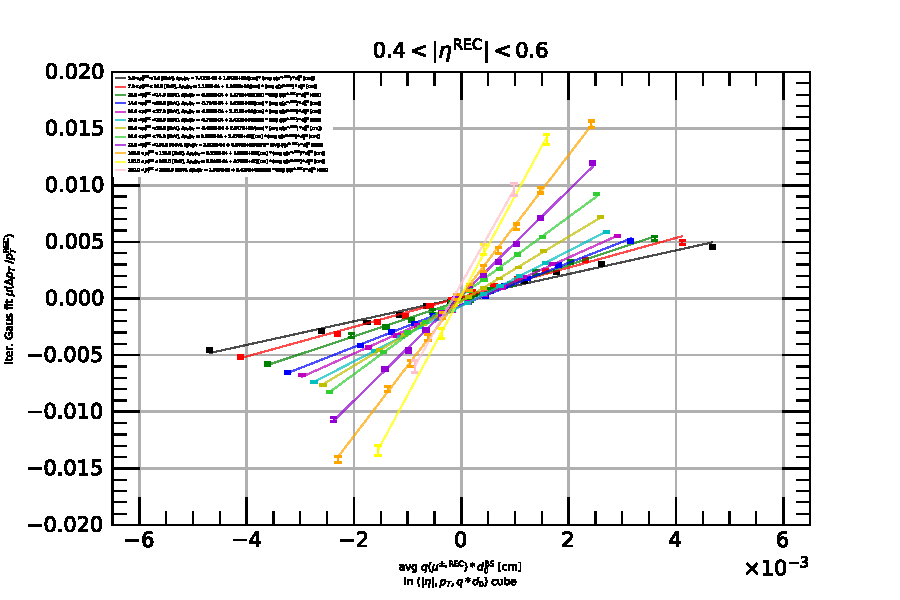
\includegraphics[height=4cm]{../../higgsmassmeasurement/AN-19-248/Figures/adhoc_d0/dpToverpTvsqd0_graphs_2018/graph_dpTvsqd0_0p4eta0p6.png}}
%     { 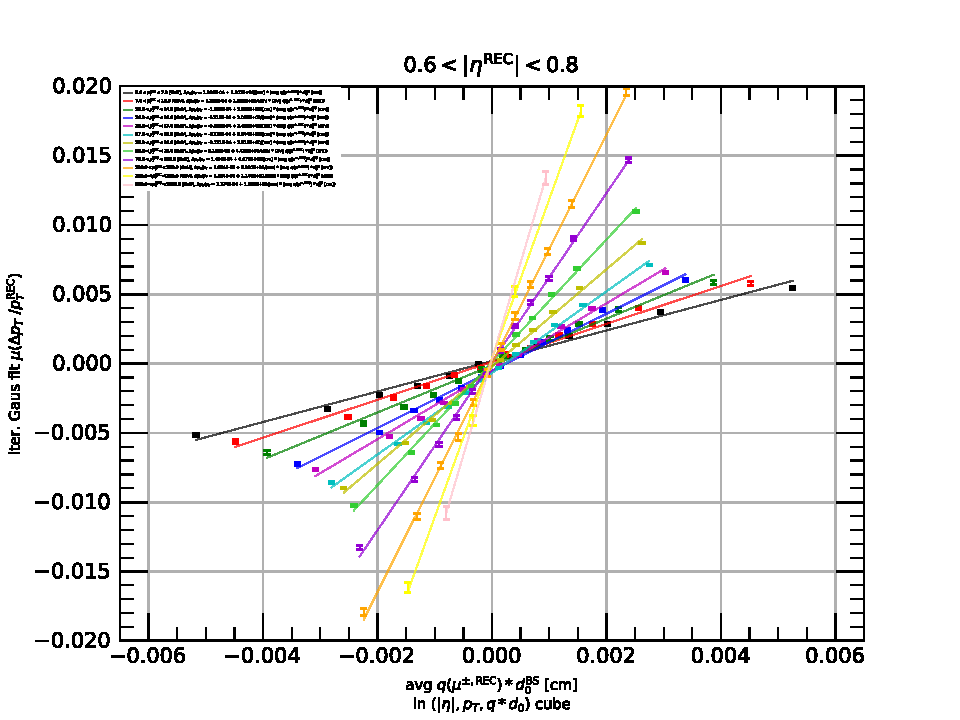
\includegraphics[height=4cm]{../../higgsmassmeasurement/AN-19-248/Figures/adhoc_d0/dpToverpTvsqd0_graphs_2018/graph_dpTvsqd0_0p6eta0p8.png}}
%     { 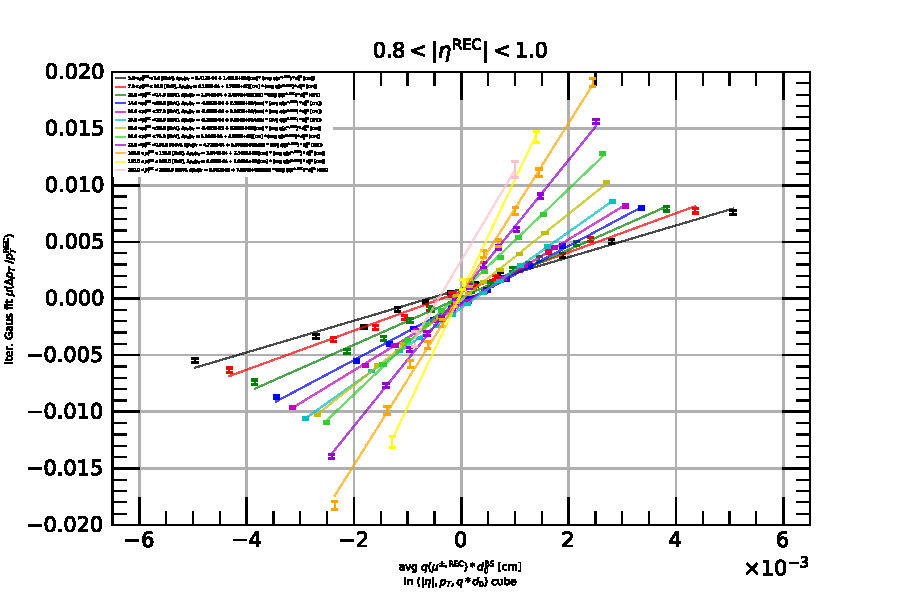
\includegraphics[height=4cm]{../../higgsmassmeasurement/AN-19-248/Figures/adhoc_d0/dpToverpTvsqd0_graphs_2018/graph_dpTvsqd0_0p8eta1p0.png}}
%     { \includegraphics[height=4cm]{../../higgsmassmeasurement/AN-19-248/Figures/adhoc_d0/dpToverpTvsqd0_graphs_2018/graph_dpTvsqd0_1p0eta1p3.png}}
%     { \includegraphics[height=4cm]{../../higgsmassmeasurement/AN-19-248/Figures/adhoc_d0/dpToverpTvsqd0_graphs_2018/graph_dpTvsqd0_1p3eta1p5.png}}
%     \caption
%         [Graphs of \pTmismeas vs. avg$(\qdzero)$ for 2018 MC: bins = [0.0, 0.2, 0.4, 0.6, 0.8, 1.0, 1.25, 1.5].]
%         { 
%         Graphs of \pTmismeas vs. avg$(\qdzero)$ for each \abseta bin using 2018 MC.
%         The \abseta bin edges shown above are: $[0.0, 0.2, 0.4, 0.6, 0.8, 1.0, 1.25, 1.5]$.
%         Each line uses data from a single \pT bin. 
%         The \pT correction parameters for each (\abseta, \pT) bin are found in the legend.
%         }
% \end{figure}
% \newpage
% % TODO: Make multiFigure
% \begin{figure}[!htbp]
%     % \vspace*{0.3cm}
%     \centering
%     { \includegraphics[height=4cm]{../../higgsmassmeasurement/AN-19-248/Figures/adhoc_d0/dpToverpTvsqd0_graphs_2018/graph_dpTvsqd0_1p5eta1p8.png}}
%     { \includegraphics[height=4cm]{../../higgsmassmeasurement/AN-19-248/Figures/adhoc_d0/dpToverpTvsqd0_graphs_2018/graph_dpTvsqd0_1p8eta2p0.png}}
%     { \includegraphics[height=4cm]{../../higgsmassmeasurement/AN-19-248/Figures/adhoc_d0/dpToverpTvsqd0_graphs_2018/graph_dpTvsqd0_2p0eta2p1.png}}
%     { \includegraphics[height=4cm]{../../higgsmassmeasurement/AN-19-248/Figures/adhoc_d0/dpToverpTvsqd0_graphs_2018/graph_dpTvsqd0_2p1eta2p2.png}}
%     { \includegraphics[height=4cm]{../../higgsmassmeasurement/AN-19-248/Figures/adhoc_d0/dpToverpTvsqd0_graphs_2018/graph_dpTvsqd0_2p2eta2p3.png}}
%     { \includegraphics[height=4cm]{../../higgsmassmeasurement/AN-19-248/Figures/adhoc_d0/dpToverpTvsqd0_graphs_2018/graph_dpTvsqd0_2p3eta2p4.png}}
%     \caption
%         [Graphs of \pTmismeas vs. avg$(\qdzero)$ for 2018 MC: bins = [1.5, 1.75, 2.0, 2.1, 2.2, 2.3, 2.4].]
%         { 
%         Graphs of \pTmismeas vs. avg$(\qdzero)$ for each \abseta bin using 2018 MC.
%         The \abseta bin edges shown above are: $[1.5, 1.75, 2.0, 2.1, 2.2, 2.3, 2.4]$.
%         Each line uses data from a single \pT bin. 
%         The \pT correction parameters for each (\abseta, \pT) bin are found in the legend.
%     }
% \end{figure}